\subsection{Hardware}
The smart wheelchair must sense the environment, process this information,
and maneuver within the environment. Doing so requires hardware, including a
sensor system, compute unit, and motor controller.

The literature review compares several types of sensors and manufacturers for these sensors.
An RGB-D camera was selected for this application, as they provide high-resolution images and depth
information at a commercially viable price point. High-resolution image data builds flexibility into
the system, as popular machine learning algorithms can be utilised.

This RGB-D camera must be mounted to the wheelchair at an appropriate point. The front of the
joystick control unit was selected for the reasons below:
\begin{enumerate}[topsep=0pt,itemsep=-1ex,partopsep=1ex,parsep=1ex]
    \item A clear view of the environment in front of the wheelchair is provided.
    \item The user does not obstruct the camera's view in any wheelchair configuration.
    \item The camera does not obstruct the user's view or comfort in any wheelchair configuration.
    \item When exiting the wheelchair, the user can move the joystick control unit and camera
            out of the way using the existing joystick control unit mount.
\end{enumerate}
Some considerations must be addressed when using this mounting point.
\begin{enumerate}[topsep=0pt,itemsep=-1ex,partopsep=1ex,parsep=1ex]
    \item Unstable video footage could be observed due to low rigidity in the joystick control unit mount.
    \item Mount point is \SI{790}{\milli\metre} forward from the back of the wheelchair, impacting
            the visibility of the rear and side of the wheelchair.
    \item Doorway maneuverability is impacted if RGB-D camera width exceeds \SI{150}{\milli\metre}.
\end{enumerate}
This sensor mounting point is positioned on the right-hand side of the wheelchair,
\SI{720}{\milli\metre} above the ground and \SI{300}{\milli\metre} behind the
front of the wheelchair (measured from the footplate), and can be seen in \cref{fig:wheelchair_zed_1}.

The RGB-D camera model selected was the Stereolabs ZED Mini, which uses passive stereo-vision
to generate a depth map. Active IR RGB-D cameras were not viable for this application
due to their poor outdoor performance and range. The width of the ZED Mini also fulfils the
size requirements of the selected mounting point.

Smart wheelchair applications such as wheelchair docking require
obstacle detection on all sides of the wheelchair. To satisfy this requirement, a
Cygbot CygLiDAR D1 was procured for short-range detection of obstacles at the rear of the
wheelchair. Nicolas Lee, a project student focused on
wheelchair navigation to personal vehicles, selected this sensor. It should be noted that
this sensor was not used for navigation assistance as part of this thesis.

% Sensor mount design
A 3D printed sensor mount was designed to fix the ZED Mini to the wheelchair mounting point.
This sensor mount was based on a ZED Mini mount designed by Walter Lucetti at Stereolabs \cite{lucettiStereolabsZEDMini2018},
with several major modifications made using Autodesk Inventor:
\begin{enumerate}[topsep=0pt,itemsep=-1ex,partopsep=1ex,parsep=1ex]
    \item Width of the mount was greatly reduced to improve maneuverability.
    \item A mounting plate was added, allowing the sensor mount to bolt onto
            the existing joystick control unit.
    \item Some sensor clips were modified to make sensor removal more convenient.
    \item Sharp corners were rounded to reduce the risk of injury to a user.
\end{enumerate}
\Cref{fig:zed_mount} shows a render of the ZED Mini camera and custom mount.
\Cref{fig:wheelchair_zed_1} shows the ZED Mini camera mounted to the joystick control unit
on the wheelchair.

\begin{figure}[b]
    \centering
    \begin{minipage}[b]{.4\textwidth}
      \centering
      \captionsetup{width=.8\textwidth}
      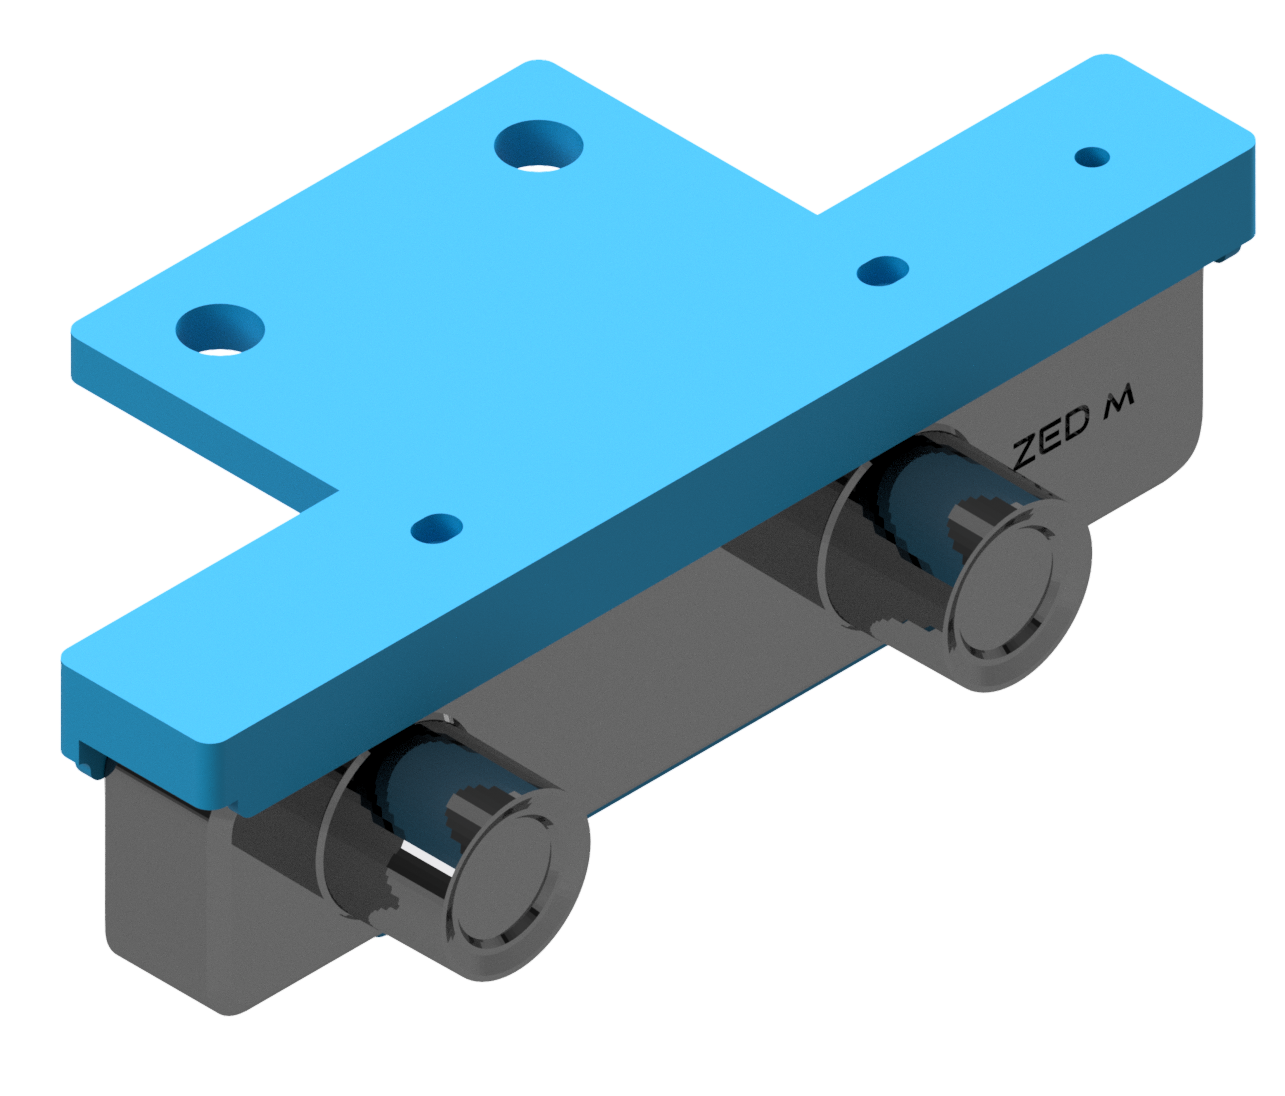
\includegraphics[width=\linewidth]{images/zed_mount.png}
        \captionof{figure}{3D render of ZED Mini camera and wheelchair mount}
        \label{fig:zed_mount}
    \end{minipage}%
    \begin{minipage}[b]{.48\textwidth}
        \centering
        \captionsetup{width=.8\textwidth}
        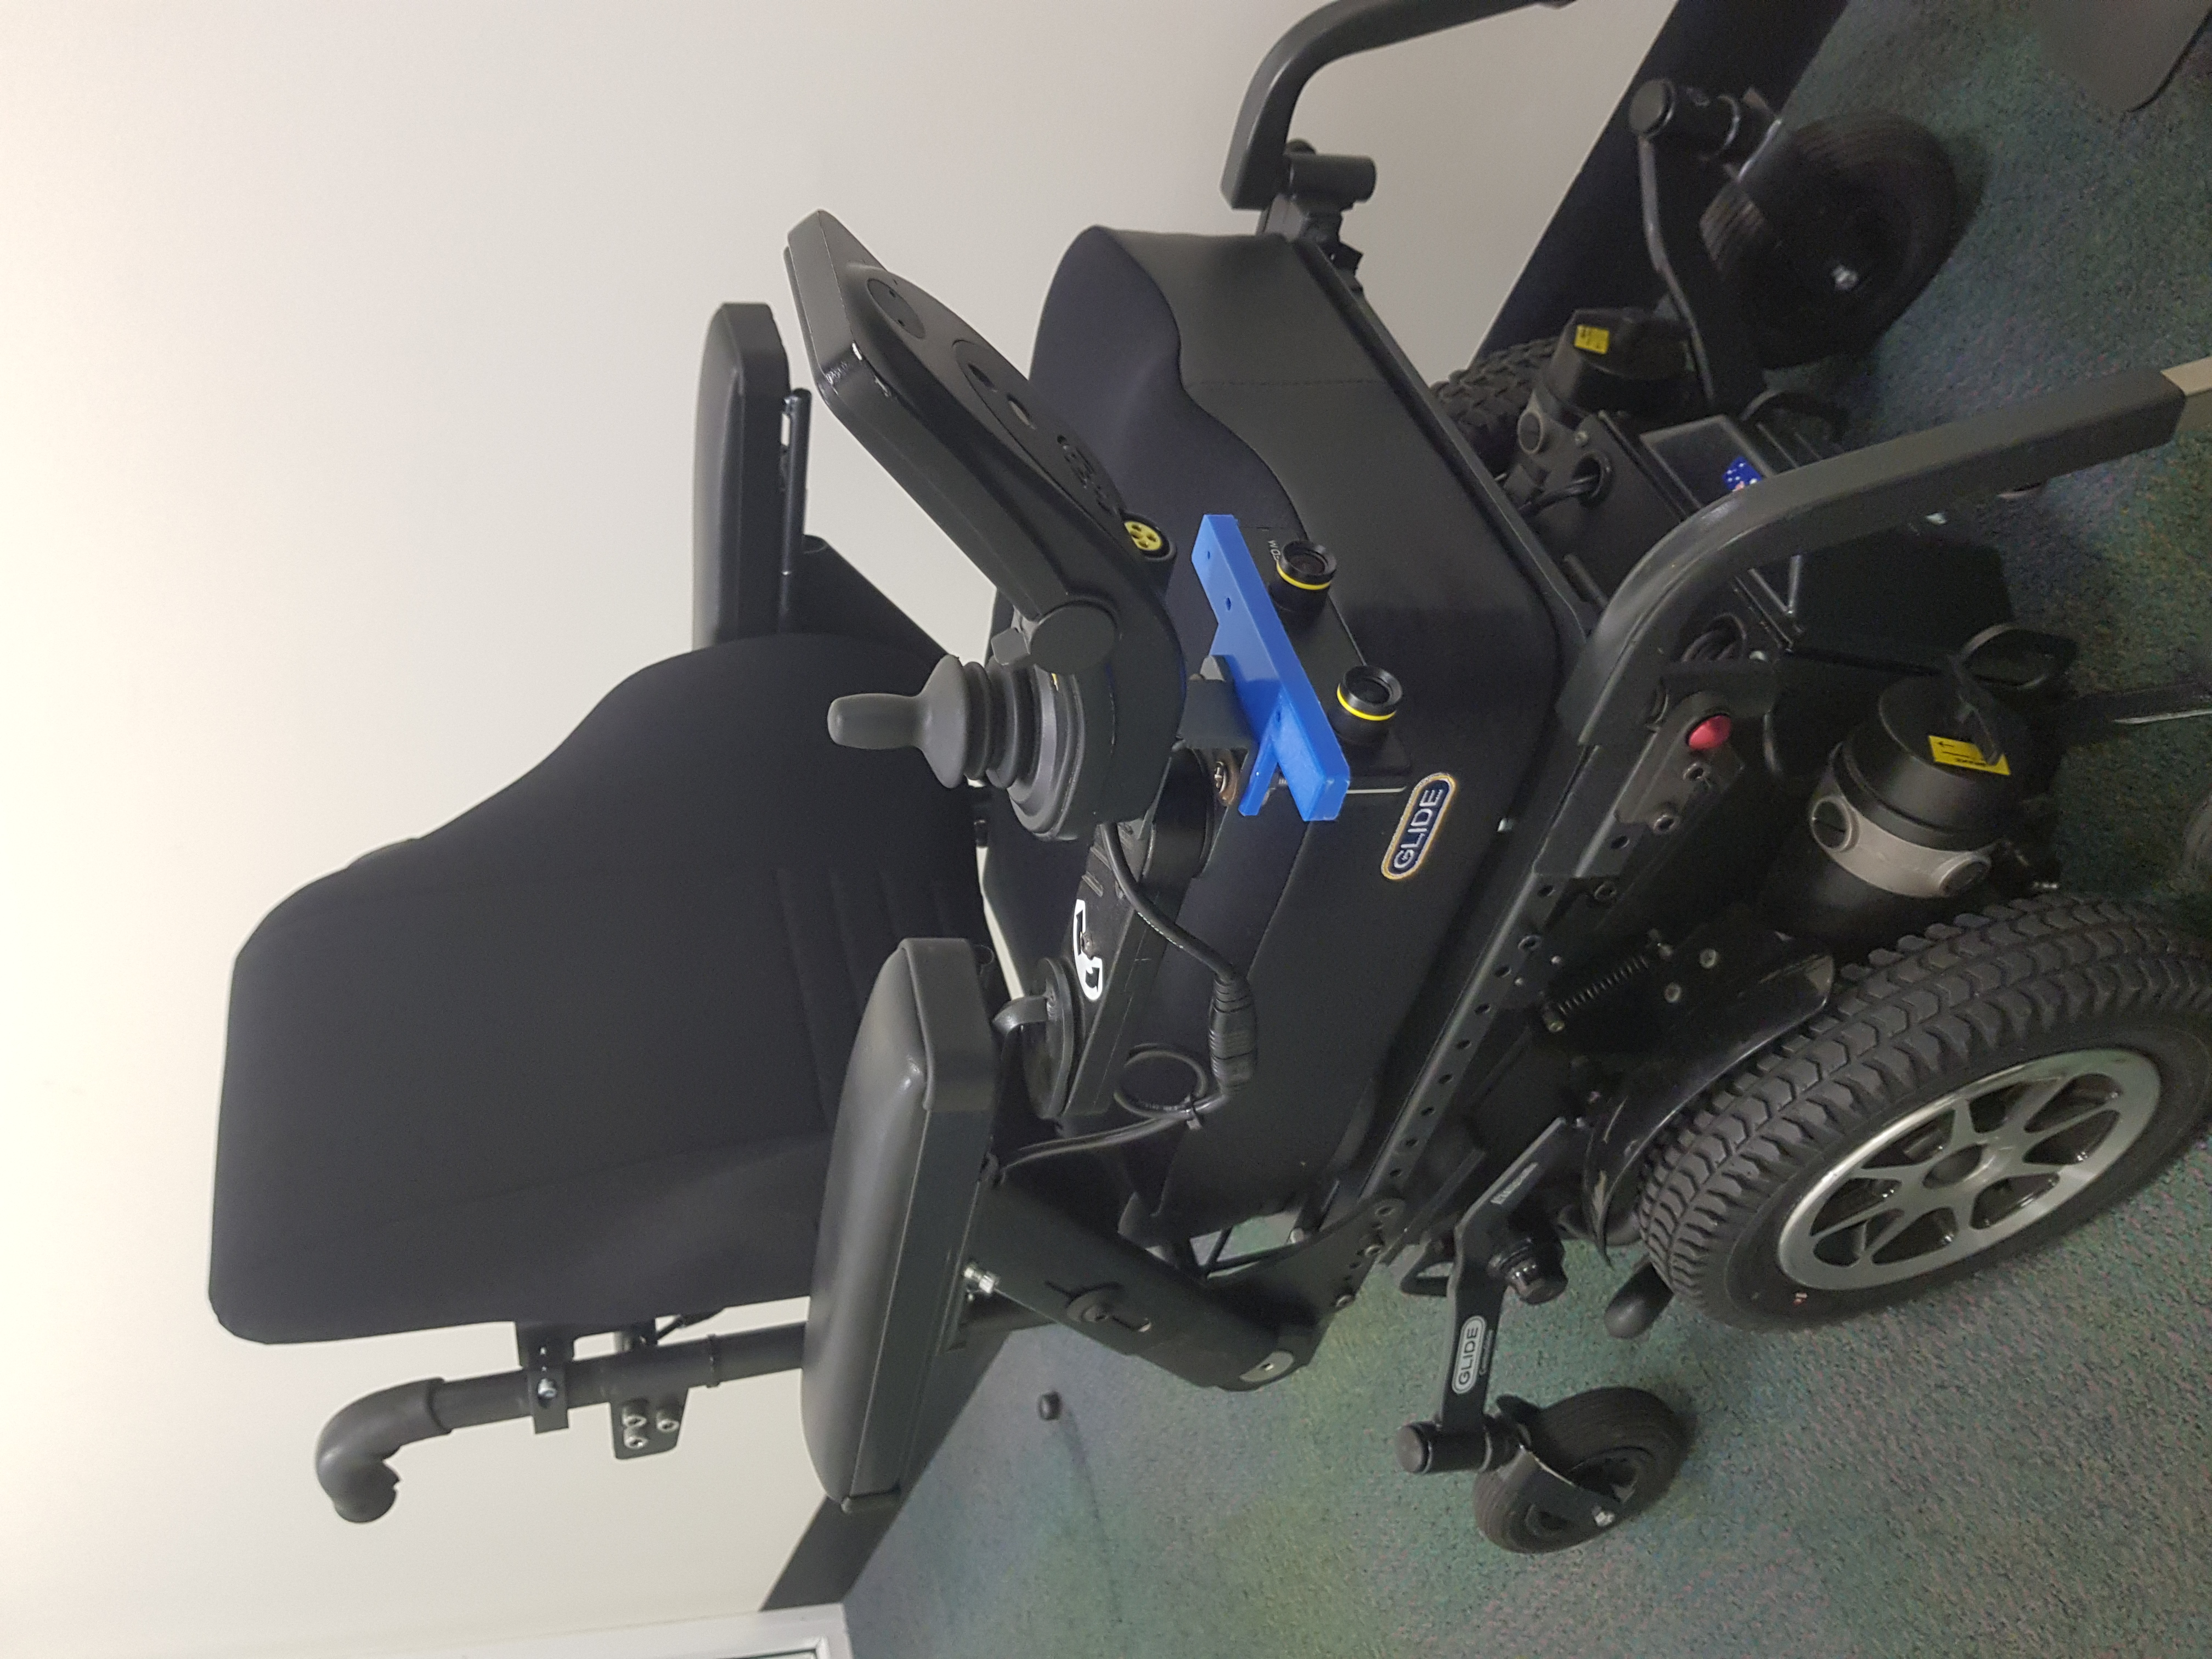
\includegraphics[height=\linewidth,angle=270,origin=c]{images/wheelchair_zed_1.jpg}
        \captionof{figure}{ZED Mini camera and mount fixed to joystick control unit}
        \label{fig:wheelchair_zed_1}
    \end{minipage}
\end{figure}

In addition to the RGB-D camera and Lidar sensor, an AI accelerator is required to process the sensors'
output and run ML algorithms. The literature review compares several AI accelerators across categories
such as computational speed, power draw, and price. An Nvidia Jetson Xavier NX was selected for this task,
as the Stereolabs ZED Mini requires a CUDA-enabled accelerator to generate a depth map. This accelerator's
low power draw and small form factor are suited for mobile robot applications such as smart wheelchairs.
Due to budget constraints and the ongoing chip shortage, the project team could not procure this AI accelerator.
Instead, a laptop with an RTX 3080 graphics card was used to record datasets and evaluate the speed of
ML algorithms.

A CentroGlide powered wheelchair was used as a base for the smart wheelchair functionality.
The CentroGlide is a mid-wheel drive wheelchair with two independently controlled powered wheels and four
unpowered castor wheels.
A joystick module communicates user commands to a power module, which controls
each motor. An intelligent seating module (ISM) adjusts the seat tilt and recline \cite{glideCentroGlideOWNERUSER2022}.
This wheelchair is \SI{1100}{\milli\metre} in length (including footplate), \SI{620}{\milli\metre}
in width, and \SI{1030}{\milli\metre} in height.
Communication between the joystick module, power module, and ISM is shown in \cref{fig:module_communication}.

\begin{figure}[b]
    \centering
    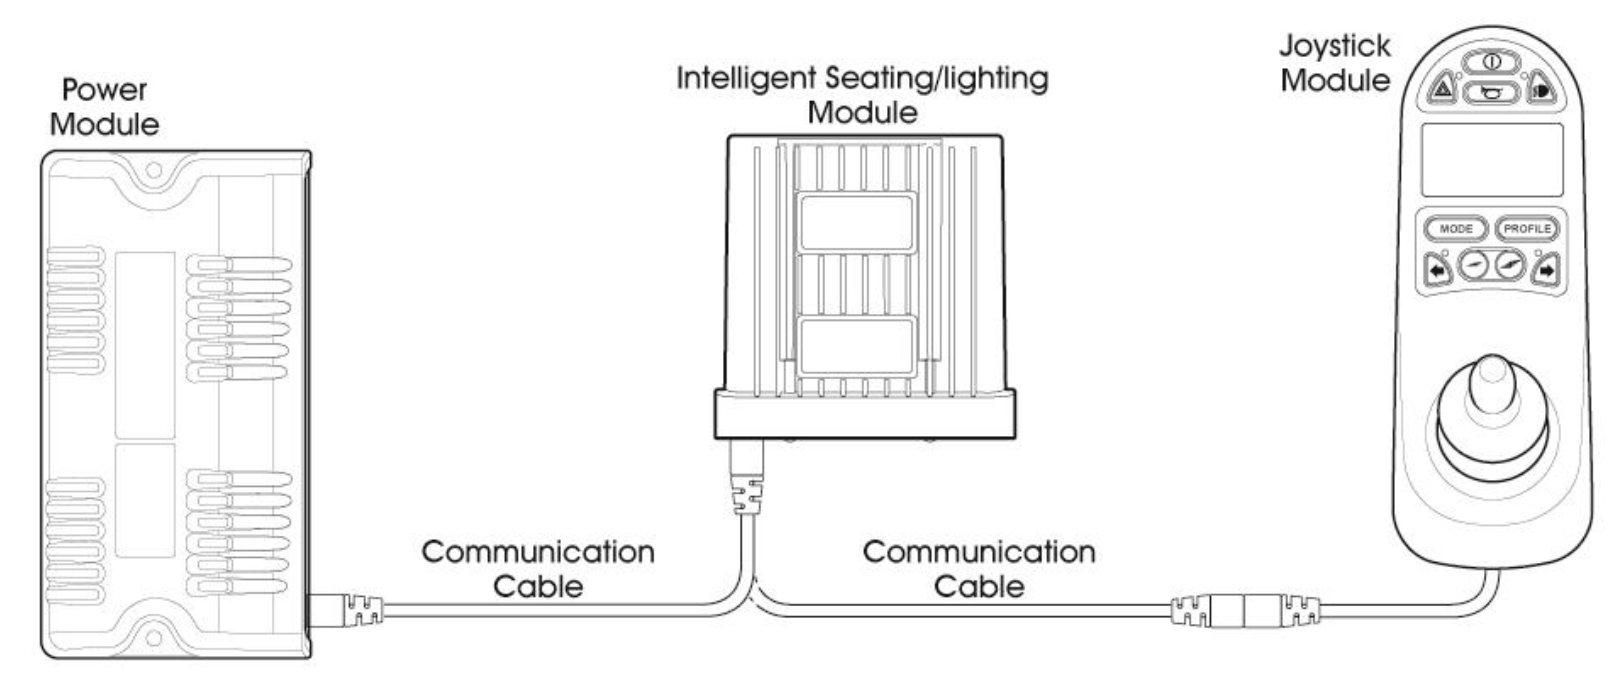
\includegraphics[width=0.7\linewidth]{images/module_communication.png}
    \caption{Communication between CentroGlide control modules. Reproduced from Curtiss-Wright. \cite{curtiss-wrightPGDRIVESTECHNOLOGY2016}}
    \label{fig:module_communication}
\end{figure}

An input controller is being developed by project student Brian Smith to intercept
commands from the joystick module and communicate with the smart wheelchair navigation system.
The input controller enables the navigation system to receive user commands and choose a safe
direction and speed for the wheelchair.
A high-level protocol between the navigation system and input controller has been designed
and is detailed in the future work section of this thesis. The input controller will validate the
navigation system's output, ensuring that the user
can still safely maneuver the wheelchair in the case of a software failure.
Additionally, a motor controller was developed by project student
Kosma Egan, which receives commands from the input controller to drive and monitor the motors.
\pagebreak

\subsection{Software}
The software system involves several scene recognition algorithms to update an internal
map of the surrounding area, keeping track of suitable driving paths and static obstacles
such as walls and stairs. Once this map is created, an algorithm blends the
user's input with this information to determine a safe path forward.
All relevant code can be found on \href{https://github.com/JakobWyatt/smart-wheelchair}{\underline{Github}}.

First, the ZED SDK is used to communicate with the ZED Mini camera and retrieve image data,
point cloud data, and depth map data. Next, several scene recognition algorithms
identify drivable areas and environmental obstacles. A block diagram of the software system
and how it interacts with the hardware is shown in \cref{fig:block_diagram}.

\begin{figure}[b]
    \centering
    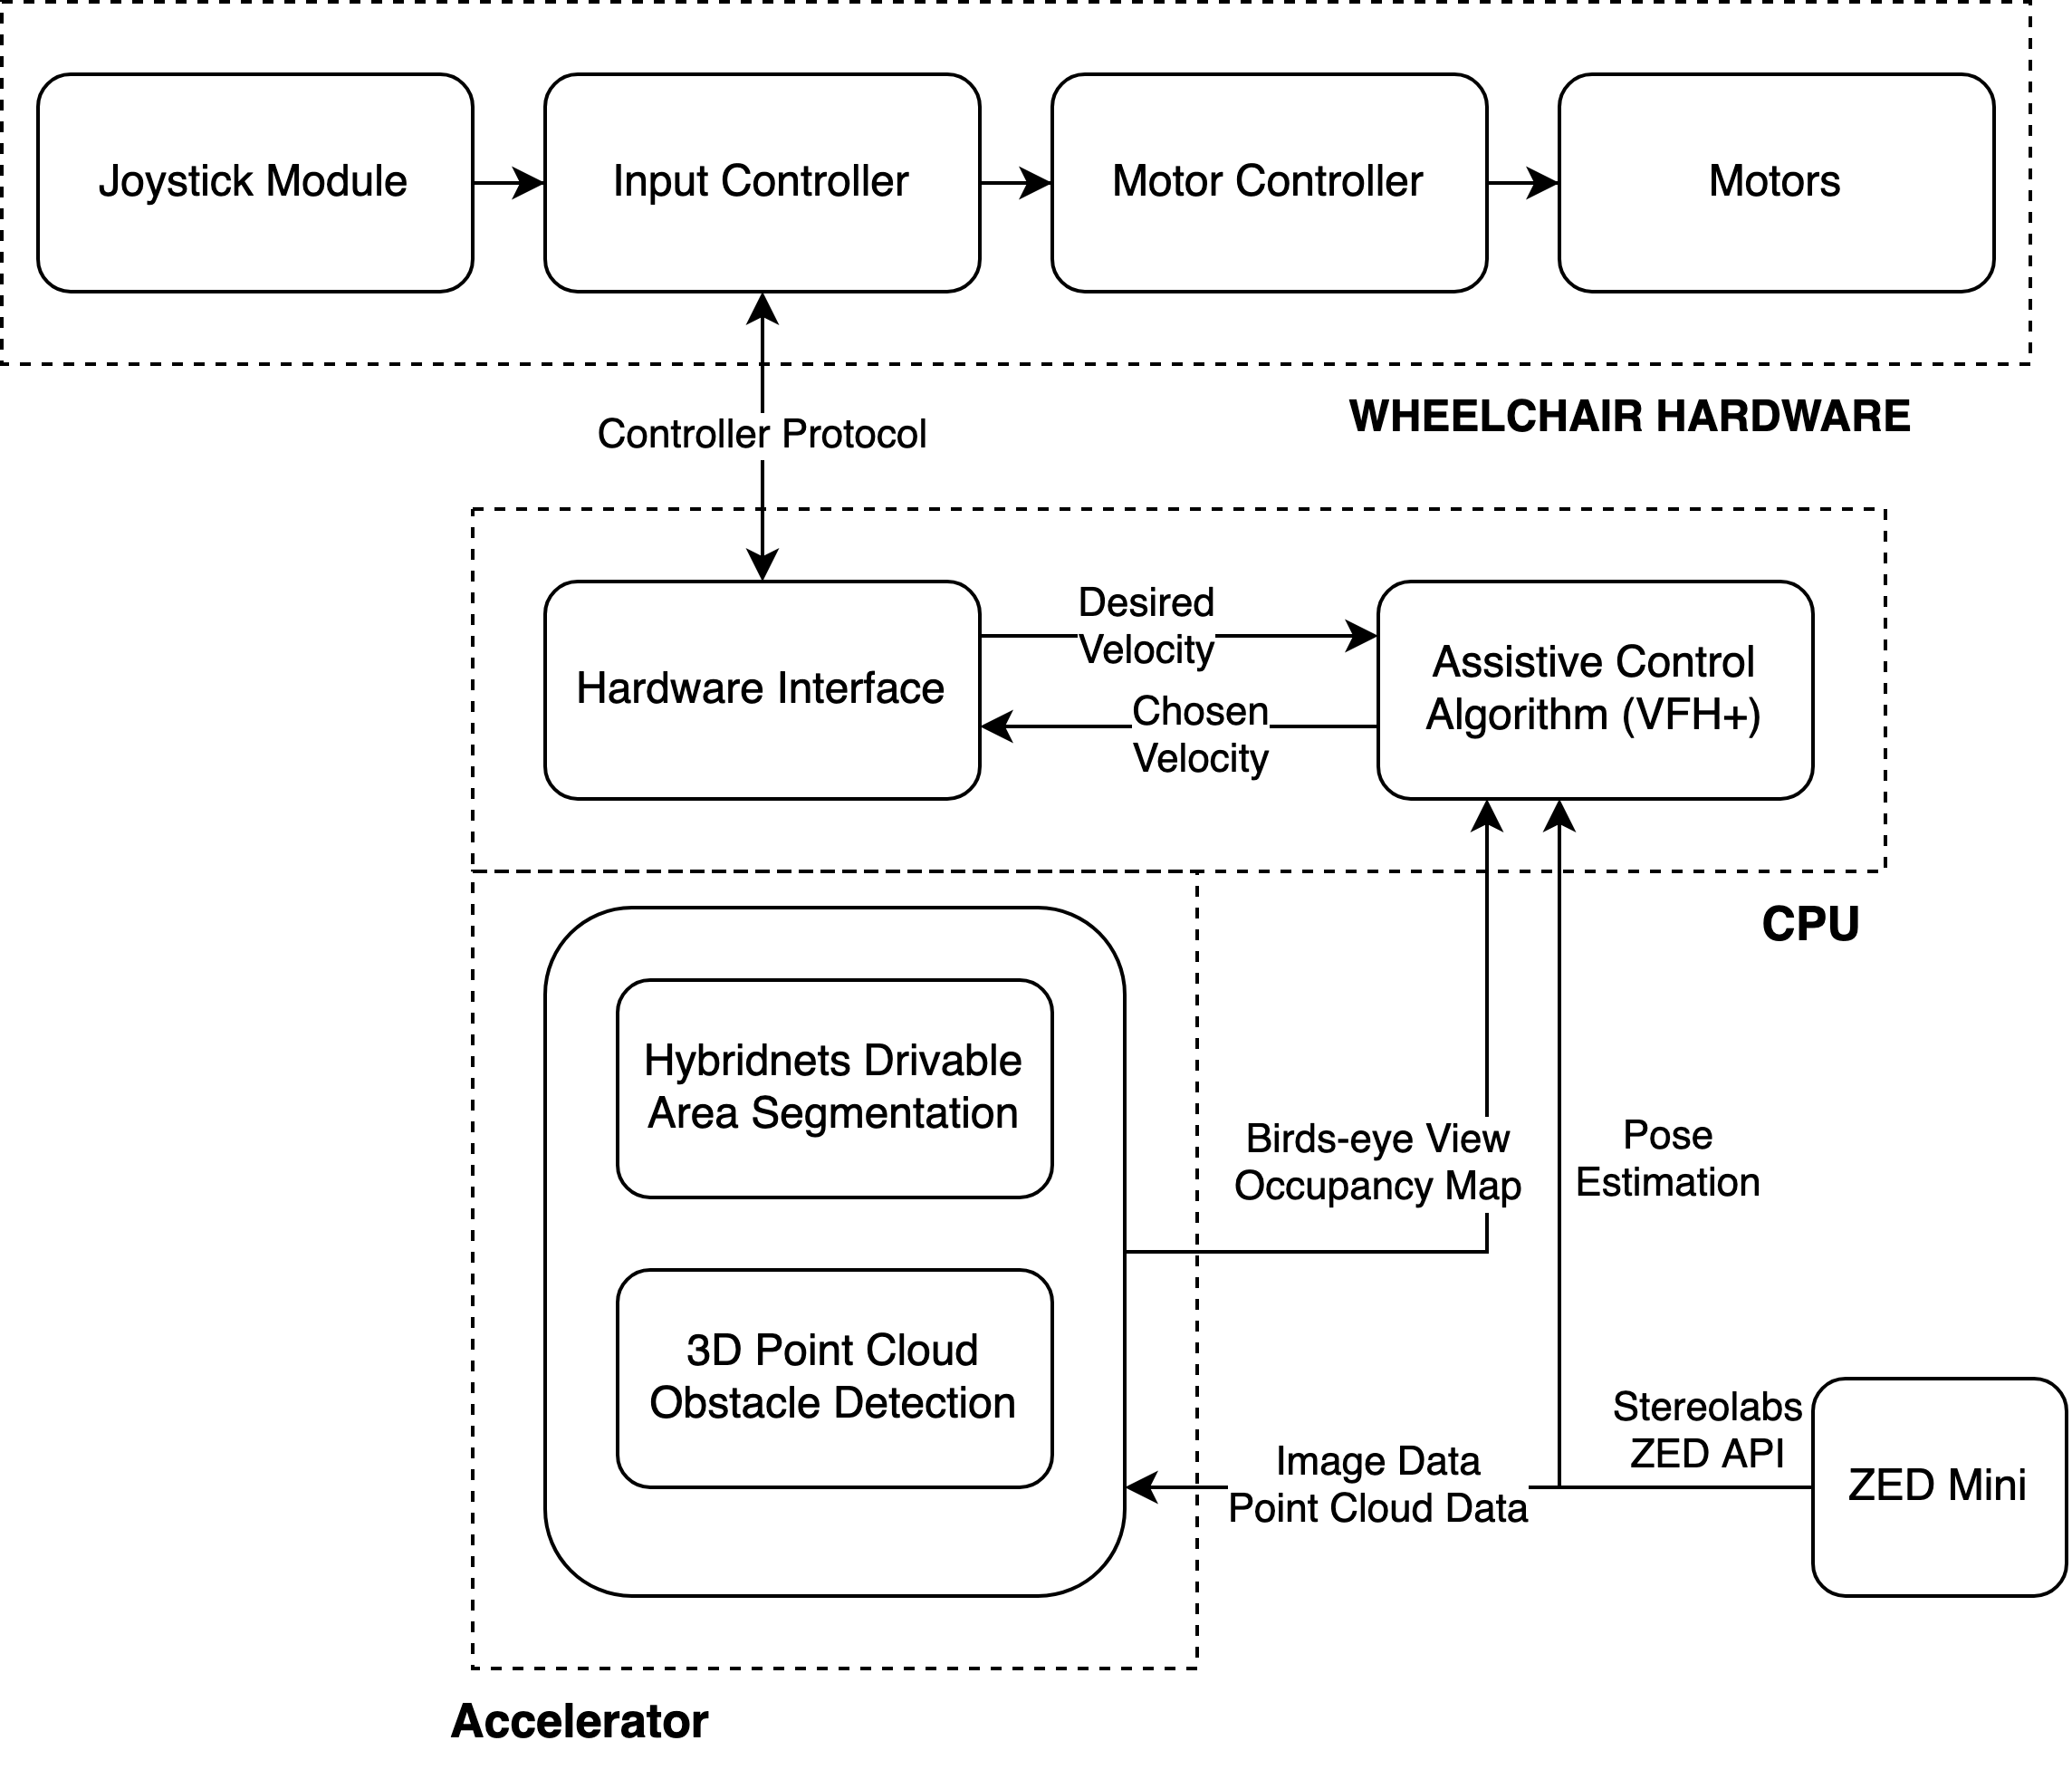
\includegraphics[width=0.9\linewidth]{images/block_diagram.png}
    \caption{Block diagram of software system and interaction with hardware components}
    \label{fig:block_diagram}
\end{figure}

Hybridnets \cite{vuHybridNetsEndtoEndPerception2022},
a machine learning model which performs drivable area segmentation and object detection on the same
image recognition backbone, was trained and evaluated on the Berkely Deepdrive dataset \cite{yuBDD100KDiverseDriving2018}
and the Cityscapes dataset \cite{cordtsCityscapesDatasetSemantic2016}. This model was used to identify
which areas were suitable for the wheelchair user to drive on,
and as a proof of concept for a shared-backbone model architecture.
Object detection models such as YOLOv5 \cite{ultralyticsYOLOv5} and image segmentation models such as
DeepLabv3 \cite{chenRethinkingAtrousConvolution2017} were evaluated and compared to Hybridnets using a preliminary
video-only wheelchair driving dataset.
Machine learning was done using PyTorch \cite{paszkePyTorchImperativeStyle2019}, due to good compatibility
with existing machine learning models.

The 3D point cloud data was used to identify the corresponding location of a drivable segmented pixel in 3D space.
This data was used to build a birds-eye view occupancy map of the local area, extending \SI{15}{\metre}
in front of the wheelchair and \SI{5}{\metre} on either side.
Large numerical computations were done using Numpy due to efficiency and ease of use.

Morphological image processing techniques were used to improve the density of the occupancy map.
The OpenCV \cite{bradskiOpenCVLibrary2000} implementation of morphological dilation was used to
join the space between drivable pixels, to create a continuous driving surface in the occupancy map
rather than many separate pixels.

Manual processing of the 3D point cloud data was also tested to identify the floor plane and drivable area.
This approach was compared with the inbuilt \texttt{find\_floor\_plane} ZED API function.
Environmental obstacles between the heights of \SI{0.5}{\metre} and \SI{2.0}{\metre} were
detected using the 3D point cloud data and added to the occupancy map.

% MATLAB camera -> center of wheelchair transform?
The VFH+ (vector field histogram) algorithm \cite{ulrichVFHReliableObstacle1998} was used to blend
the user's desired direction with the occupancy map to determine a safe target direction.
This algorithm was implemented in MATLAB using the Navigation toolbox. The `MATLAB Engine' API
was used to transfer data between Python and MATLAB code.
As the input controller had not been implemented yet, joystick commands could not be logged; instead,
the user's desired direction was assumed to be the current direction of the wheelchair.

The ZED Sensors API and ZED Positional Tracking API were tested to track the movement of the wheelchair.
The Sensors API performs pose estimation using 6 DOF IMU sensor fusion and can also output raw accelerometer
and gyroscope data. The Positional Tracking API combines sensor data with image data to track the camera's movement.

\subsection{Dataset Collection}
An RGB-D wheelchair driving dataset was collected around Curtin university
to test and evaluate the performance of the navigation assistance system.
This dataset is \SI{7.14}{\giga\byte} in size and \SI{47}{\minute} in length
and includes features such as indoor and outdoor navigation, doorways, pedestrians,
elevator use, wheelchair access ramps, and car parks. This dataset can be accessed at the
\href{https://curtin.sharepoint.com/:f:/r/sites/CurtinXGlide/Shared%20Documents/Navigation%20and%20Object%20Detection/ZED?csf=1&web=1&e=tTau9D}{\underline{Curtin X Glide (Smart Wheelchair)}} Teams channel.

This dataset was collected using the ZED Mini and is encoded in the proprietary Stereolabs SVO file format, which can be read using the ZED SDK.
This format includes image data from left and right cameras, IMU data, and metadata such as
timestamps. Depth map and point cloud data are not stored in the dataset and are instead generated when
the file is read using the ZED SDK.

Four compression modes are available during dataset collection: Lossless (PNG), Lossy (JPG), H.264 (Video),
and H.265. Both video compression modes require a CUDA-enabled device during dataset collection.
A 10-second sample dataset was recorded for each compression mode to evaluate image quality and
file size (results in \cref{table:dataset_compression_modes}).

Due to the smaller file size, H.264 compression was used when collecting the wheelchair driving dataset.
\Cref{fig:zed_sample_dataset} shows an example image frame and depth map from the dataset.

In addition to the RGB-D dataset, a preliminary wheelchair driving video-only dataset was collected around
Curtin university \href{https://curtin.sharepoint.com/:v:/r/sites/CurtinXGlide/Shared%20Documents/Navigation%20and%20Object%20Detection/GoPro%20Dataset.mp4?csf=1&web=1&e=seLdRb}{\underline{(also hosted on teams)}}.
This dataset was \SI{34}{\minute} in length and \SI{7.08}{\giga\byte} in size (1920x1080 @ 24 fps)
and collected using a GoPro Hero 4.
This dataset was used to evaluate machine learning scene recognition algorithms
before the ZED Mini had been ordered.

%\vspace{4.0cm}

\begin{table}[H]
    \centering
    \begin{tabular}{c c c c}
    \toprule
    Compression mode & File size & Relative increase & Image quality \\
    \midrule
    Lossless (PNG) & \SI{1240}{\mega\byte} & 41 & Ok \\
    Lossy (JPG) & \SI{640}{\mega\byte} & 21 & Some interlacing \\
    H.264 & \SI{30}{\mega\byte} & 1 & OK \\
    H.265 & \SI{30}{\mega\byte} & 1 & Some frame tearing \\
    \bottomrule
    \end{tabular}
    \caption{Comparison between dataset compression modes}
    \label{table:dataset_compression_modes}
\end{table}

\begin{figure}[b]
    \centering
    \begin{subfigure}{.48\textwidth}
        \centering
        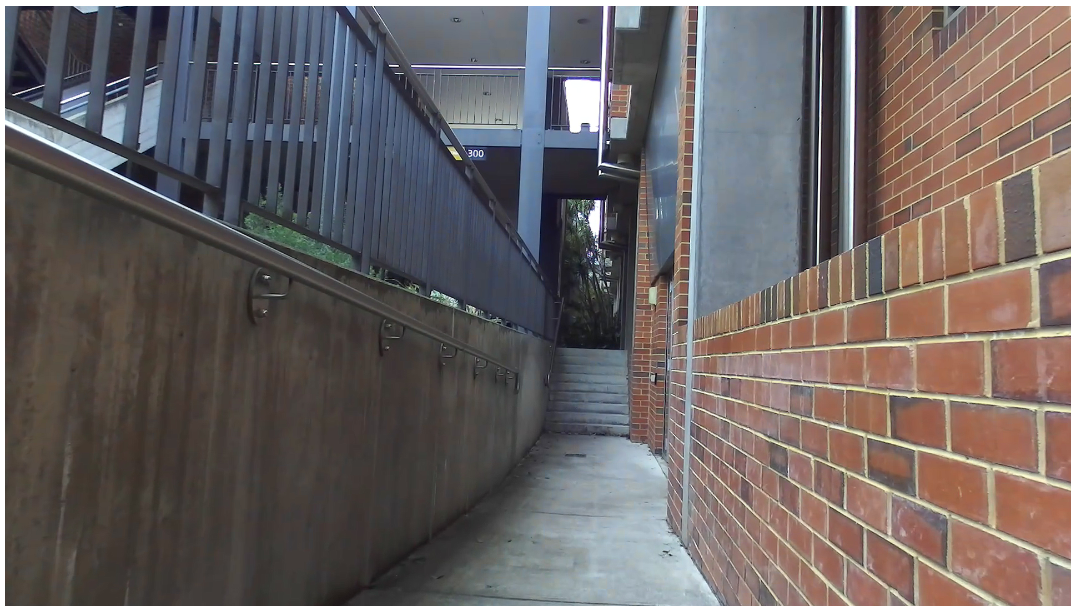
\includegraphics[width=\linewidth]{images/zed_sample_image.png}
        \caption{Image frame}
    \end{subfigure}
    \quad
    \begin{subfigure}{.47\textwidth}
        \centering
        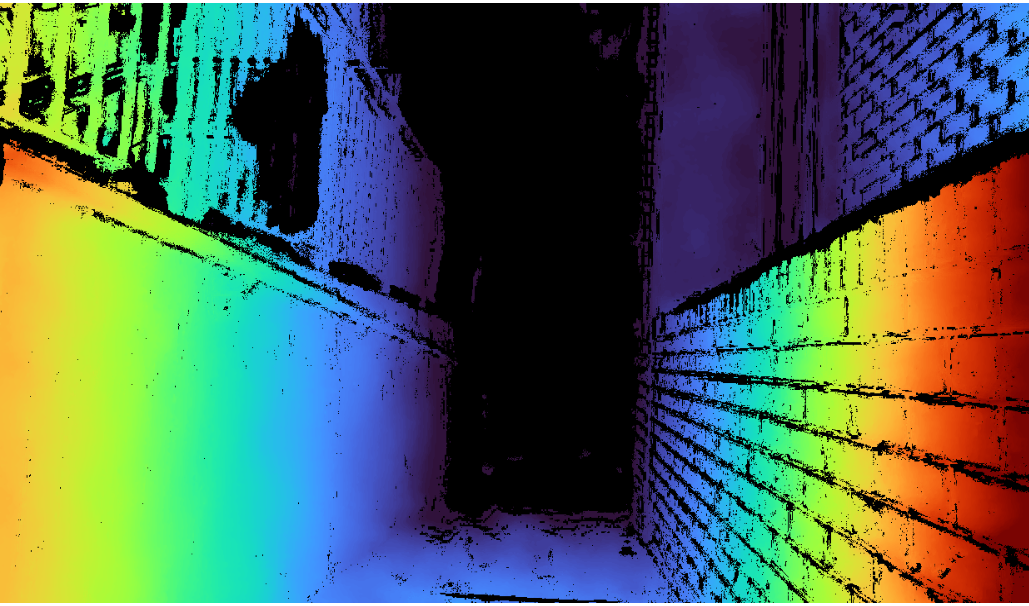
\includegraphics[width=\linewidth]{images/zed_sample_depth.png}
        \caption{Depth map}
    \end{subfigure}
    \caption{Sample data from the Curtin university RGB-D wheelchair driving dataset}
    \label{fig:zed_sample_dataset}
\end{figure}
